\section{Particle kinematics}
In Sec.~\ref{sec:ltqs} we discussed 4-momentum and how
it transform under a Lorentz-boost. One important point
is that energy and momentum conservation still applies. These
conservation rules are different to frame invariance, and rather
refer to conservation in time ie
\[
E_{\rm TOTAL}=E_{1}+E_{2}+...+E_{n}
\]
and 
\[
\vec{p}_{\rm TOTAL}=\vec{p}_{1}+\vec{p}_{2}+...+\vec{p}_{n},
\]
are both conserved quantities at any point in space and time.
However:
\[
m_{\rm TOTAL}=m_{1}+m_{2}+...+m_{n},
\]
is NOT conserved, but IS invariant under Lorentz transformations.

\noindent Let us consider a couple of applications of energy-momentum conservation
in particle collisions. In particle physics,
\noindent 
\[
m^{2}=p_{\rm TOTAL}\cdot p_{\rm TOTAL}=E^{2}_{\rm TOTAL}-\vec{p}^{2}_{\rm TOTAL},
\]

is used to quantify the energy involved in a collision. As $m^{2}$ is a Lorentz invariant quantity, 
it is equivalent to the total energy squared in a frame where $\vec{p}^{2}_{\rm TOTAL}=0$ 
i.e the Centre of Mass (CoM) frame. Therefore we can define $s\equiv m^2$ and  thus $\sqrt{s}$ is the CoM energy.

\paragraph{Example 1: ``Fixed target'' collision}
\begin{center}
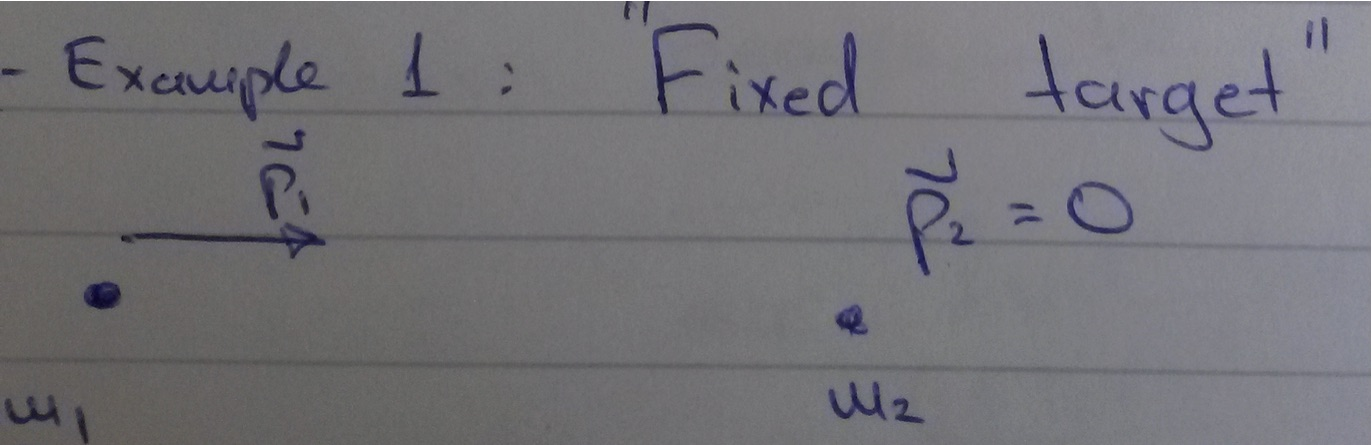
\includegraphics[width=0.5\textwidth]{fig/collisions/collisions_example1.jpg}
\end{center}

In this example
\[
s=(E_{1}+E_{2})^{2}-(\vec{p_1})^2.
\]
since $\vec{p_2}=\vec{0}$. Remembering 
that $|p_1|^2=E_{1}^{2}-m_{1}^{2}$ (using natural units) and rearranging, we get
\[
E_{1}=\frac{s-m_{1}^{2}-m_{2}^{2}}{2m_{2}}.
\]
\noindent Therefore in a fixed target collision, in order to achieve a CoM 
energy $\sqrt{s}$, one needs a beam of energy as given above.  If we make the assumption that the required $s$ is much larger than $m_{1}^2$ and $m_{2}^{2}$, then the expression for the beam energy of a fixed target collider reduces to\footnote{Particle beams
consist of electrons or protons or pions or kaons. All these particles have masses $<1$~GeV.
The mass of the target does not refer to the macroscopic mass of the whole target block, but rather to the microscopic mass of nucleus with which the proton interacts. For all practical purposes the mass of the target can be considered as the atomic mass of the nucleus. Depending on the target, the mass can vary between $\sim 1$~GeV for a hydrogen target to $\mathcal{O}(10)$~GeV for a beryllium target or $\mathcal{O}(100)$~GeV for a molybdenum target.}:
\begin{equation}
\label{eq:e_fixed_target}
E_{1}\sim \frac{s}{2m_{2}}.
\end{equation}

\paragraph{Example 2: ``Particle collider''}
\begin{center}
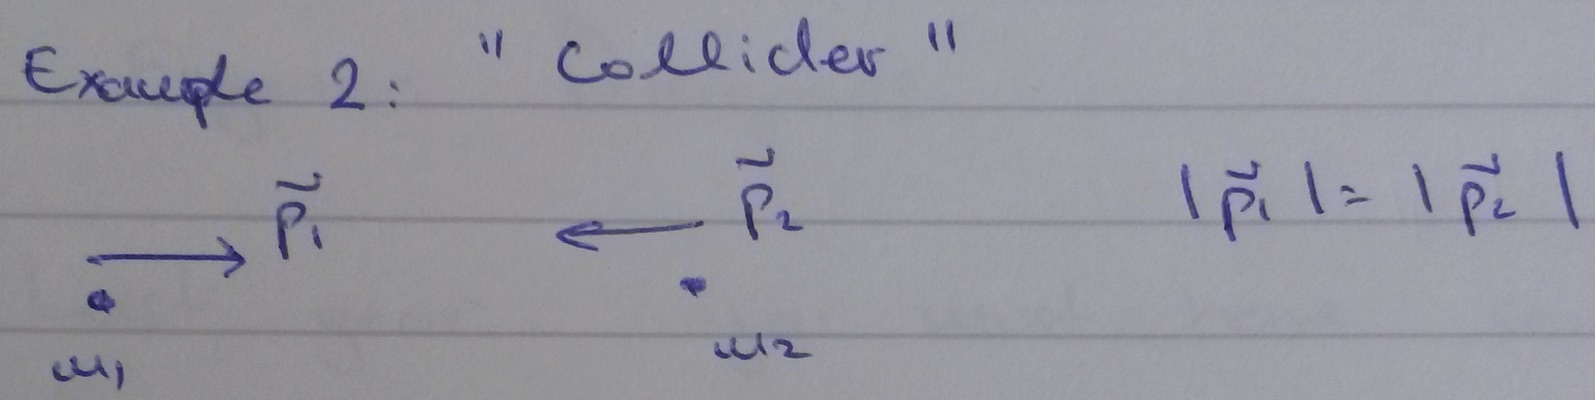
\includegraphics[width=0.5\textwidth]{fig/collisions/collisions_example2.jpg}
\end{center}
Consider two colliding beams with $\vec{p_1}=-\vec{p_2}$.
In this case:
\[
s=(E_{1}+E_{2})^{2}.
\]
Using  $|p_1|^2=|p_2|^2$ we have:
\[
E_{1}^{2}-E_{2}^{2}=m_{1}^{2}-m_{2}^{2}
\]
Therefore we can replace $E_2$ in favour of $E_1$ and get:
\[
E_1=\frac{s+m_{1}^{2}-m_{2}^{2}}{2\sqrt{s}}
\]
Under the assumption that $s \gg m_{1}^2,m_{2}^2$, we can write:
\begin{equation}
\label{eq:e_collider}
E_{1}\sim \frac{\sqrt{s}}{2}.
\end{equation}

Consider now that we want to build an accelarator which produces collisions
at $\sqrt{s}=13$000~GeV (13~TeV), very much like the Large Hadron Collider running
currently at CERN. Given Eq.~\ref{eq:e_collider}, one would require a beam energy of 6.5~TeV per beam. 

If however we were to use a ``fixed-target'' type facility, then using Eq.~\ref{eq:e_fixed_target}, where we consider a hydrogen target in which case $m_{2}\sim 1$~GeV, the required beam energy would be $E_{1}=\frac{13000^2}{2\times1}\sim84.5$~PeV!!

These two examples illustrate why if one is after high energies, it is much more efficient to accelerate and collide two beams rather than whack a single beam onto a target. If however one is interested in a large number of collisions (high intensity rather than high energy) then the most efficient way is a ``fixed target'' configuration.

\exercise{
When the Large Hadron Collider started colliding beams at $\sqrt{s}=13$~TeV, some members of the press claimed that: ``The Large Hadron Collider produces the highest energy collisions in our solar system ''. 

Cosmic rays are high energy charged particles originating outside our solar system. They have been observed to have energies up to $10^{20}$~eV. By considering the collision of the most energetic cosmic ray with stationary hydrogen gas in the universe decide whether the statement was correct.
\rotatebox{180}{Answer: Cosmic ray on Hydrogen $\sqrt{s}\sim450$~TeV.
%Hydrogen gas means the target particle is\\ a proton of mass $m_p\sim 1$~GeV. So for a fixed target collision we have $\sqrt{s}\sim\sqrt{2E m_p}$ Therefore $\sqrt{s}\sim\sqrt{1\times10^{20}\times1\times10^9}\sim450~$~TeV,\newline compared to LHC's 13~TeV so the statement was incorrect.
}
}
